% (find-LATEX "2020-2-C2-P2.tex")
% (defun c () (interactive) (find-LATEXsh "lualatex -record 2020-2-C2-P2.tex" :end))
% (defun C () (interactive) (find-LATEXsh "lualatex 2020-2-C2-P2.tex" "Success!!!"))
% (defun D () (interactive) (find-pdf-page      "~/LATEX/2020-2-C2-P2.pdf"))
% (defun d () (interactive) (find-pdftools-page "~/LATEX/2020-2-C2-P2.pdf"))
% (defun e () (interactive) (find-LATEX "2020-2-C2-P2.tex"))
% (defun o () (interactive) (find-LATEX "2020-2-C2-P2.tex"))
% (defun u () (interactive) (find-latex-upload-links "2020-2-C2-P2"))
% (defun v () (interactive) (find-2a '(e) '(d)))
% (defun d0 () (interactive) (find-ebuffer "2020-2-C2-P2.pdf"))
% (defun cv () (interactive) (C) (ee-kill-this-buffer) (v) (g))
%          (code-eec-LATEX "2020-2-C2-P2")
% (find-pdf-page   "~/LATEX/2020-2-C2-P2.pdf")
% (find-sh0 "cp -v  ~/LATEX/2020-2-C2-P2.pdf /tmp/")
% (find-sh0 "cp -v  ~/LATEX/2020-2-C2-P2.pdf /tmp/pen/")
%     (find-xournalpp "/tmp/2020-2-C2-P2.pdf")
%   file:///home/edrx/LATEX/2020-2-C2-P2.pdf
%               file:///tmp/2020-2-C2-P2.pdf
%           file:///tmp/pen/2020-2-C2-P2.pdf
% http://angg.twu.net/LATEX/2020-2-C2-P2.pdf
% (find-LATEX "2019.mk")
% (find-CN-aula-links "2020-2-C2-P2" "2" "c2m202p2" "c2p2")
%
% Video:
% (find-ssr-links "c2m202p2" "2020-2-C2-P2")
% (code-video     "c2m202p2video" "$S/http/angg.twu.net/eev-videos/2020-2-C2-P2.mp4")
% (find-c2m202p2video "0:00")

% «.defs»		(to "defs")
% «.defs-T-and-B»	(to "defs-T-and-B")
% «.title»		(to "title")
% «.regras-e-dicas»	(to "regras-e-dicas")
% «.questao-1»		(to "questao-1")
% «.questao-1-dicas»	(to "questao-1-dicas")
% «.questao-1-dicas-2»	(to "questao-1-dicas-2")
% «.questao-1-figura»	(to "questao-1-figura")
% «.questao-1-extras»	(to "questao-1-extras")
% «.questao-2»		(to "questao-2")
%
% «.djvuize»		(to "djvuize")

\documentclass[oneside,12pt]{article}
\usepackage[colorlinks,citecolor=DarkRed,urlcolor=DarkRed]{hyperref} % (find-es "tex" "hyperref")
\usepackage{amsmath}
\usepackage{amsfonts}
\usepackage{amssymb}
\usepackage{pict2e}
\usepackage[x11names,svgnames]{xcolor} % (find-es "tex" "xcolor")
\usepackage{colorweb}                  % (find-es "tex" "colorweb")
%\usepackage{tikz}
%
% (find-dn6 "preamble6.lua" "preamble0")
\usepackage{proof}   % For derivation trees ("%:" lines)
\input diagxy        % For 2D diagrams ("%D" lines)
\xyoption{curve}     % For the ".curve=" feature in 2D diagrams
%
\usepackage{edrx15}               % (find-LATEX "edrx15.sty")
\input edrxaccents.tex            % (find-LATEX "edrxaccents.tex")
\input edrxchars.tex              % (find-LATEX "edrxchars.tex")
\input edrxheadfoot.tex           % (find-LATEX "edrxheadfoot.tex")
\input edrxgac2.tex               % (find-LATEX "edrxgac2.tex")
%
%\usepackage[backend=biber,
%   style=alphabetic]{biblatex}            % (find-es "tex" "biber")
%\addbibresource{catsem-slides.bib}        % (find-LATEX "catsem-slides.bib")
%
% (find-es "tex" "geometry")
\usepackage[a6paper, landscape,
            top=1.5cm, bottom=.25cm, left=1cm, right=1cm, includefoot
           ]{geometry}
%
\begin{document}

\catcode`\^^J=10
\directlua{dofile "dednat6load.lua"}  % (find-LATEX "dednat6load.lua")

% %L dofile "edrxtikz.lua"  -- (find-LATEX "edrxtikz.lua")
% %L dofile "edrxpict.lua"  -- (find-LATEX "edrxpict.lua")
% \pu

% «defs»  (to ".defs")
% (find-LATEX "edrx15.sty" "colors-2019")
\long\def\ColorRed   #1{{\color{Red1}#1}}
\long\def\ColorViolet#1{{\color{MagentaVioletLight}#1}}
\long\def\ColorViolet#1{{\color{Violet!50!black}#1}}
\long\def\ColorGreen #1{{\color{SpringDarkHard}#1}}
\long\def\ColorGreen #1{{\color{SpringGreenDark}#1}}
\long\def\ColorGreen #1{{\color{SpringGreen4}#1}}
\long\def\ColorGray  #1{{\color{GrayLight}#1}}
\long\def\ColorGray  #1{{\color{black!30!white}#1}}
\long\def\ColorBrown #1{{\color{Brown}#1}}
\long\def\ColorBrown #1{{\color{brown}#1}}
\long\def\ColorOrange#1{{\color{orange}#1}}

\long\def\ColorShort #1{{\color{SpringGreen4}#1}}
\long\def\ColorLong  #1{{\color{Red1}#1}}

\def\frown{\ensuremath{{=}{(}}}
\def\True {\mathbf{V}}
\def\False{\mathbf{F}}
\def\D    {\displaystyle}

\def\drafturl{http://angg.twu.net/LATEX/2020-2-C2.pdf}
\def\drafturl{http://angg.twu.net/2020.2-C2.html}
\def\draftfooter{\tiny \href{\drafturl}{\jobname{}} \ColorBrown{\shorttoday{} \hours}}

\def\pfo #1{\ensuremath{\mathsf{[#1]}}}

% «defs-T-and-B»  (to ".defs-T-and-B")
% (c3m202p1p 6 "questao-2")
% (c3m202p1    "questao-2")
\def\T(Total: #1 pts){{\bf(Total: #1)}}
\def\T(Total: #1 pts){{\bf(Total: #1 pts)}}
\def\T(Total: #1 pts){\ColorRed{\bf(Total: #1 pts)}}
\def\B       (#1 pts){\ColorOrange{\bf(#1 pts)}}



%  _____ _ _   _                               
% |_   _(_) |_| | ___   _ __   __ _  __ _  ___ 
%   | | | | __| |/ _ \ | '_ \ / _` |/ _` |/ _ \
%   | | | | |_| |  __/ | |_) | (_| | (_| |  __/
%   |_| |_|\__|_|\___| | .__/ \__,_|\__, |\___|
%                      |_|          |___/      
%
% «title»  (to ".title")
% (c2m202p2p 1 "title")
% (c2m202p2    "title")

\thispagestyle{empty}

\begin{center}

\vspace*{1.2cm}

{\bf \Large Cálculo 2 - 2020.2}

\bsk

P2 (segunda prova)

\bsk

Eduardo Ochs - RCN/PURO/UFF

\url{http://angg.twu.net/2020.2-C2.html}

\end{center}

\newpage

% «regras-e-dicas»  (to ".regras-e-dicas")
% (c2m202p2p 2 "regras-e-dicas")
% (c2m202p2    "regras-e-dicas")

As regras e dicas são as mesmas dos mini-testes e da P1:

\ssk

\url{http://angg.twu.net/LATEX/2020-2-C2-MT1.pdf}

\url{http://angg.twu.net/LATEX/2020-2-C2-MT2.pdf}

\url{http://angg.twu.net/LATEX/2020-2-C2-P1.pdf}

\ssk

exceto que a prova vai ser disponibilizada às 21:00 do dia

29/abril/2021 e deve ser entregue até as 22:00 do dia

30/abril/2021.

\newpage

% «questao-1»  (to ".questao-1")
% (c2m202p2p 3 "questao-1")
% (c2m202p2    "questao-1")
% (c2m202stp 1 "title")
% (c2m202st    "title")

{\bf Questão 1.}

\T(Total: 6.5+1.5 pts)

Na parte do curso sobre substituição trigonométrica --- link:

\ssk

{\footnotesize

\url{http://angg.twu.net/LATEX/2020-2-C2-subst-trig.pdf}

}

\ssk

você aprendeu a demonstrar fórmulas de integração, a dar nomes pra
elas, a criar uma ``tabela de integrais'' sua só com fórmulas que você
sabe demonstrar, e a usar as fórmulas da sua tabela de integrais.
Agora você vai demonstrar duas fórmulas sobre substituição
trigonométrica que não vimos nas aulas e que vão ser usadas algumas
vezes nos cursos de Física.

Lembre que várias fórmulas de integração importantes não resolvem
integrais, só convertem elas pra integrais mais fáceis de resolver.
Várias fórmulas do slides de substituição trigonométrica são assim, e
as que você vai demonstrar aqui também vão ser.

\newpage

{\bf Questão 1 (cont.)}

\msk

a) \B(2.0 pts) Demonstre uma fórmula como esta aqui,
%
$$\intx{x^α \sqrt{a^2 x^2 - 1}^β} = \ColorRed{k}
  \intu{u^α \sqrt{    u^2 - 1}^β}
$$

e dê um nome para ela. Você vai ter que descobrir qual é a

substituição certa e qual é o valor da expressão $\ColorRed{k}$. Obs: $a>0$.


\msk

b) \B(2.0 pts) Demonstre uma fórmula como esta aqui,
%
$$\intx{x^α \sqrt{x^2 - b^2}^β} = \ColorRed{w}
  \intu{u^α \sqrt{u^2 - 1  }^β}
$$

e dê um nome para ela. Você vai ter que descobrir qual é a

substituição certa e qual é o valor da expressão $\ColorRed{w}$. Obs: $b>0$.

\newpage

{\bf Questão 1 (cont.)}

\msk

c) \B(2.5 pts) Demonstre uma fórmula como esta aqui,
%
$$\intx{x^α \sqrt{a^2x^2 - b^2}^β} = \ColorRed{z}
  \intu{u^α \sqrt{   u^2 - 1  }^β}
$$

e dê um nome para ela. Você vai ter que descobrir qual é a

substituição certa e qual é o valor da expressão $\ColorRed{z}$.

Obs: $a,b>0$.


\newpage

% «questao-1-dicas»  (to ".questao-1-dicas")
% (c2m202p2p 6 "questao-1-dicas")
% (c2m202p2    "questao-1-dicas")
% (find-books "__analysis/__analysis.el" "hernandez")
% (find-hernandezpage (+ 10  53) "7 Substituição trigonométrica")

{\bf Dicas pra questão 1}

Tente generalizar isto aqui,
%
$$\def\P#1{\left(#1\right)}
  \sqrt{x^2 - 25}
  \;=\; \sqrt{25 \P{\P{\frac x5}^2 - 1}}
  \;=\; 5 \sqrt{\P{\frac x5}^2 - 1} \;,
$$

e se você precisar de mais idéias veja o gabarito da questão 2

aqui:

% (find-pdf-page "~/LATEX/2018-2-C2-P1.pdf" 2)
% (find-LATEX "2018-2-C2-P1.tex" "gab-2")

\ssk

{\footnotesize

\url{http://angg.twu.net/LATEX/2018-2-C2-P1.pdf}

}

\ssk

e a ``Aula 7'' das notas da Cristiane Hernández.

\msk

Além disso dê nomes para as suas fórmulas! Se você souber usar

a fórmula do item (a) pra demonstrar o item (b) e as fórmulas dos

itens (a) e (b) pra demonstrar o (c) as suas demonstrações podem

ficar bem curtas.


\newpage

% «questao-1-dicas-2»  (to ".questao-1-dicas-2")
% (c2m202p2p 7 "questao-1-dicas-2")
% (c2m202p2    "questao-1-dicas-2")

{\bf Mais dicas para a questão 1}

\ssk

Se você achar difícil demais resolver os itens (a), (b) e (c)

direto no caso geral, em que $α,β∈\Z$ e $a,b>0$, comece com

um caso particular bem simples --- por exemplo $α=0$, $β=1$,

$a=b=5$ --- depois tente outro caso particular simples,

depois outro, até você conseguir o caso geral.

\msk

Veja a figura da próxima página...

\msk

...e repare que passar do caso geral para um caso particular

é fácil --- é só fazer uma substituição, ou deletar passos

intermediários --- mas encontrar o caso geral que generaliza

vários casos particulares conhecidos é difícil.

\msk

(Ir pra baixo na figura é fácil, ir pra cima é difícil)


\newpage

% «questao-1-figura»  (to ".questao-1-figura")
% (c2m202p2p 8 "questao-1-figura")
% (c2m202p2    "questao-1-figura")

%\def\Foo#1#2{
%  \left(
%  \begin{array}{rcl}
%   2^{#2}-2^{#1} &=& 2^{1+#1}-2^{#1} \\
%   %             &=& 2^{1}·2^{#1}-2^{#1} \\
%                 &=& 2·2^{#1}-1·2^{#1} \\
%                 &=& (2-1)·2^{#1} \\
%   %             &=& 1·2^{#1} \\
%                 &=& 2^{#1} \\
%   \end{array}
%   \right)
%}

\def\Foo#1#2{
  \left(
  \begin{array}{rcl}
   2^{#1+1}-2^{#1} &=& 2^{1+#1}-2^{#1} \\
                   &=& 2^{1}·2^{#1}-2^{0}·2^{#1} \\
                   &=& 2·2^{#1}-1·2^{#1} \\
                   &=& (2-1)·2^{#1} \\
                   &=& 1·2^{#1} \\
                   &=& 2^{#1} \\
   \end{array}
   \right)
}
\def\foo#1#2{
  \left(
  \begin{array}{rcl}
   2^{#2}-2^{#1} % &=& 2^{1+#1}-2^{#1} \\
   %               &=& 2^{1}·2^{#1}-2^{#1} \\
                 % &=& 2·2^{#1}-1·2^{#1} \\
                 % &=& (2-1)·2^{#1} \\
   %               &=& 1·2^{#1} \\
                 &=& 2^{#1} \\
   \end{array}
   \right)
}

%D diagram specialize
%D 2Dx     100 +55 +55
%D 2D  100     A0
%D 2D
%D 2D  +65 A1      A2
%D 2D
%D 2D  +45 A3      A4
%D 2D
%D ren   A0   ==>     \Foo{k}{k+1}
%D ren A1  A2 ==> \Foo{4}{5}  \Foo{99}{100}
%D ren A3  A4 ==> \foo{4}{5}  \foo{99}{100}
%D
%D (( A0 A1 -> .PLABEL= _(0.55) [k:=4]
%D    A0 A2 -> .PLABEL= ^(0.55) [k:=99]
%D    A1 A3 ->
%D    A2 A4 ->
%D ))
%D enddiagram
%D
$\pu
 \scalebox{0.87}{$
 \diag{specialize}
 $}
$




\newpage

% «questao-1-extras»  (to ".questao-1-extras")
% (c2m202p2p 5 "questao-1-extras")
% (c2m202p2     "questao-1-extras")

{\bf Questão 1: itens extras}

(Acrescentados depois, a pedido dos alunos)

Sejam:
%
$$\begin{array}{rcl}
  \pfo{P2.1a} &=&
    \left( \intx{x^α \sqrt{a^2 x^2 - 1}^β} = k
           \intu{u^α \sqrt{    u^2 - 1}^β}
    \right)
    \\
  \pfo{P2.1b} &=&
    \left( \intx{x^α \sqrt{x^2 - b^2}^β} = w
           \intu{u^α \sqrt{u^2 - 1  }^β}
    \right)
    \\
  \pfo{P2.1c} &=&
    \left( \intx{x^α \sqrt{a^2x^2 - b^2}^β} = z
           \intu{u^α \sqrt{   u^2 - 1  }^β}
    \right)
    \\
  \end{array}
$$

Escreva o resultado das substituições abaixo:

\ssk

d) \B(0.1 pts) $\pfo{P2.1a} \bsm{α:=0 \\ β:=1 \\ a:=3}$

\ssk

e) \B(0.1 pts) $\pfo{P2.1b} \bsm{α:=0 \\ β:=1 \\ b:=5}$

\ssk

f) \B(0.1 pts) $\pfo{P2.1c} \bsm{α:=0 \\ β:=1 \\ a:=2 \\ b:=4}$


\newpage

{\bf Questão 1: itens extras (cont.)}

Nos itens (d), (e) e (f) do slide anterior você deve ter

obtido três igualdades novas. Vamos dar nomes pra elas. Sejam:
%
$$\begin{array}{rcl}
  \pfo{P2.1d} &:=& \pfo{P2.1a} \bsm{α:=0 \\ β:=1 \\ a:=3        } \\[7.5pt]
  \pfo{P2.1e} &:=& \pfo{P2.1b} \bsm{α:=0 \\ β:=1 \\ b:=5        } \\[7.5pt]
  \pfo{P2.1f} &:=& \pfo{P2.1c} \bsm{α:=0 \\ β:=1 \\ a:=2 \\ b:=4} \\
  \end{array}
$$

\newpage

{\bf Questão 1: itens extras (cont.)}

\msk

g) \B(0.2 pts) Encontre uma mudança de variável --- algo como,

por exemplo, $\bsm{u=42x \\ dx = \frac{1}{42}du}$ --- e um valor para
$k$ que façam a

igualdade $\pfo{P2.1d}$ ser verdade.

\msk

Agora faça a mesma coisa para as igualdades $\pfo{P2.1e}$ e $\pfo{P2.1f}$:

\msk

h) \B(0.2 pts) Encontre uma mudança de variável e um valor

para $w$ que façam a igualdade $\pfo{P2.1e}$ ser verdade.

\ssk

i) \B(0.2 pts) Encontre uma mudança de variável e um valor

para $z$ que façam a igualdade $\pfo{P2.1f}$ ser verdade.

\newpage

{\bf Questão 1: itens extras (cont.)}

Se você tiver conseguido resolver os itens (1g), (1h) e (1i)

você conseguiu resolver alguns casos particulares dos itens

(1a), (1b) e (1c)! Vamos fazer mais casos particulares...

\msk

A partir de agora ao invés de escrever ``Encontre a mudança

de variável e o valor de $k$ (ou $w$, ou $z$...) que façam a

igualdade $\pfo{Tal}$ ser verdade'' eu vou escrever só

``Resolva $\pfo{Tal}$''.

\msk


j) \B(0.2 pts) Resolva $\pfo{P2.1a} \bsm{α:=0 \\ β:=3}$.

\ssk

k) \B(0.2 pts) Resolva $\pfo{P2.1b} \bsm{α:=0 \\ β:=3}$.

\ssk

l) \B(0.2 pts) Resolva $\pfo{P2.1c} \bsm{α:=0 \\ β:=3}$.


\newpage

{\bf Questão 1: itens extras (cont.)}

Se você tiver conseguido resolver os itens anteriores

você deve ser capaz de resolver estes aqui...

\ssk

Resolva $\pfo{P2.1a} \bmat{α:=0}$,

\ssk

Resolva $\pfo{P2.1b} \bmat{α:=0}$,

\ssk

Resolva $\pfo{P2.1c} \bmat{α:=0}$.

\msk

...e com isso você deve conseguir resolver os

itens (1a), (1b) e (1c) --- que valem muitos pontos.




\newpage

% «questao-2»  (to ".questao-2")
% (c2m202edovsp 4 "campos-dirs")
% (c2m202edovs    "campos-dirs")

{\bf Questão 2.}

\T(Total: 6.0 pts)

\msk

Obs: esta questão é bem parecida com os exercícios daqui:

{\footnotesize

\url{http://angg.twu.net/LATEX/2020-2-C2-edovs.pdf}

}

\bsk

Considere esta EDO, que vamos chamar de ``$(*)$'':
%
$$\frac{dy}{dx} \; = \; - \frac{1}{2y}$$

a) \B(0.5 pts) Desenhe o campo de direções da $(*)$.

Faça tracinhos nos pontos com $x,y∈\{-2,-1,0,1,2\}$.

\msk

b) \B(1.0 pts) ``Resolva direto'' a EDO $(*)$, como no

exercício 5 dos slides.

\newpage

{\bf Questão 2 (cont.)}

\ssk

c) \B(1.0 pts) Descubra qual é a solução da $(*)$ que passa

pelo ponto $(0,2)$, e chame-a de $f_1(x)$. Desenhe o gráfico

da função $f_1(x)$ e diga o domínio dela.

\msk

d) \B(1.0 pts) Teste a sua solução $f_1(x)$ --- ou seja:

verifique que ela é uma solução de $(*)$ e que ela

passa pelo ponto $(0,2)$.

\msk

e) \B(1.5 pts) Descubra qual é a solução da $(*)$ que passa

pelo ponto $(1,-2)$, e chame-a de $f_2(x)$. Desenhe o gráfico

da função $f_2(x)$ e diga o domínio dela.

\msk

f) \B(1.0 pts) Teste a sua solução $f_2(x)$ --- ou seja:

verifique que ela é uma solução de $(*)$ e que ela

passa pelo ponto $(1,-2)$.




\newpage

\thispagestyle{empty}

\begin{center}

\vspace*{2.0cm}

{\bf \Large Gabarito}

(incompleto)

\end{center}


\newpage


% (find-latexscan-links "C2" "20210502_C2_P2_1a")
% (find-xpdf-page "~/LATEX/2020-2-C2/20210502_C2_P2_1a.pdf")
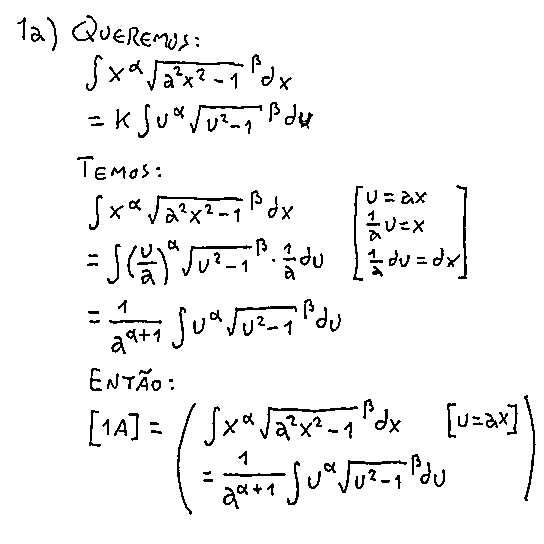
\includegraphics[height=8cm]{2020-2-C2/20210502_C2_P2_1a.pdf}

% (find-latexscan-links "C2" "20210502_C2_P2_1b")
% (find-xpdf-page "~/LATEX/2020-2-C2/20210502_C2_P2_1b.pdf")
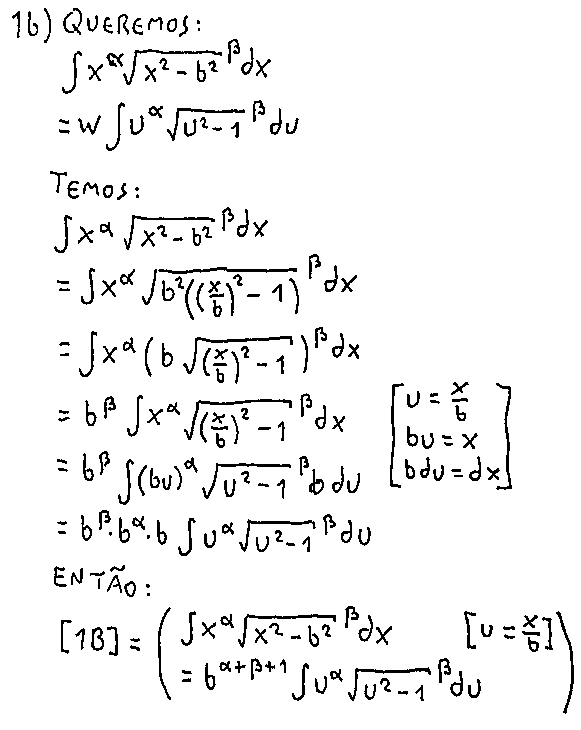
\includegraphics[height=8cm]{2020-2-C2/20210502_C2_P2_1b.pdf}

% (find-latexscan-links "C2" "20210502_C2_P2_1c")
% (find-xpdf-page "~/LATEX/2020-2-C2/20210502_C2_P2_1c.pdf")
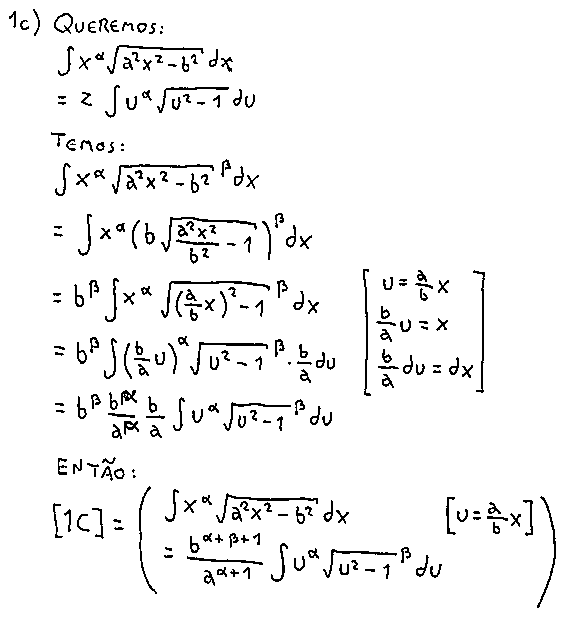
\includegraphics[height=8cm]{2020-2-C2/20210502_C2_P2_1c.pdf}


$\begin{array}[c]{c}
 % (find-latexscan-links "C2" "20210502_C2_P2_2a")
 % (find-xpdf-page "~/LATEX/2020-2-C2/20210502_C2_P2_2a.pdf")
 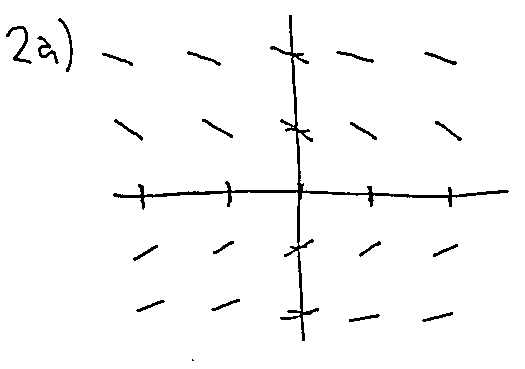
\includegraphics[height=1.75cm]{2020-2-C2/20210502_C2_P2_2a.pdf}
 \\
 % (find-latexscan-links "C2" "20210502_C2_P2_2b")
 % (find-xpdf-page "~/LATEX/2020-2-C2/20210502_C2_P2_2b.pdf")
 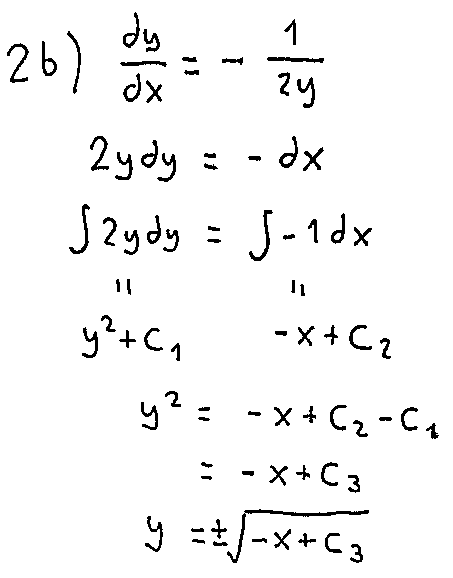
\includegraphics[height=3.0cm]{2020-2-C2/20210502_C2_P2_2b.pdf}
 \\
 % (find-latexscan-links "C2" "20210502_C2_P2_2c")
 % (find-xpdf-page "~/LATEX/2020-2-C2/20210502_C2_P2_2c.pdf")
 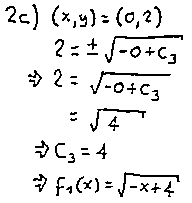
\includegraphics[height=2cm]{2020-2-C2/20210502_C2_P2_2c.pdf}
 \end{array}
 \qquad
 \begin{array}[c]{c}
 % (find-latexscan-links "C2" "20210502_C2_P2_2d")
 % (find-xpdf-page "~/LATEX/2020-2-C2/20210502_C2_P2_2d.pdf")
 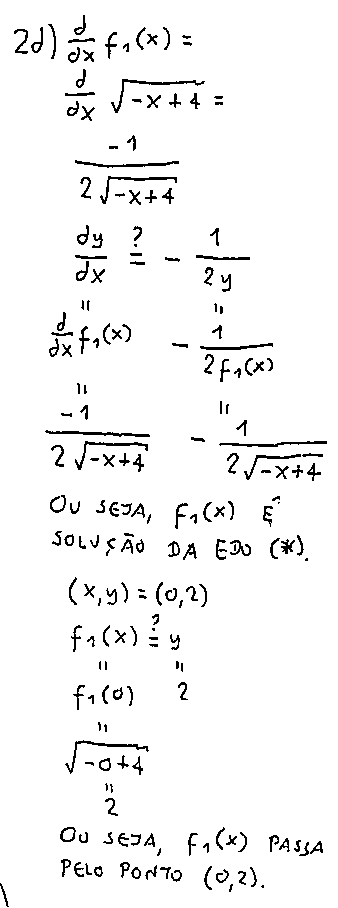
\includegraphics[height=7cm]{2020-2-C2/20210502_C2_P2_2d.pdf}
 \end{array}
$


$\begin{array}{l}
 % (find-latexscan-links "C2" "20210502_C2_P2_2e")
 % (find-xpdf-page "~/LATEX/2020-2-C2/20210502_C2_P2_2e.pdf")
 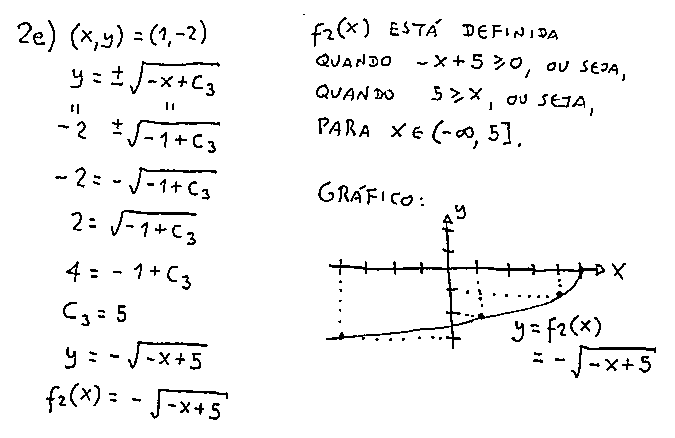
\includegraphics[height=4cm]{2020-2-C2/20210502_C2_P2_2e.pdf}
 \\
 % (find-latexscan-links "C2" "20210502_C2_P2_2f")
 % (find-xpdf-page "~/LATEX/2020-2-C2/20210502_C2_P2_2f.pdf")
 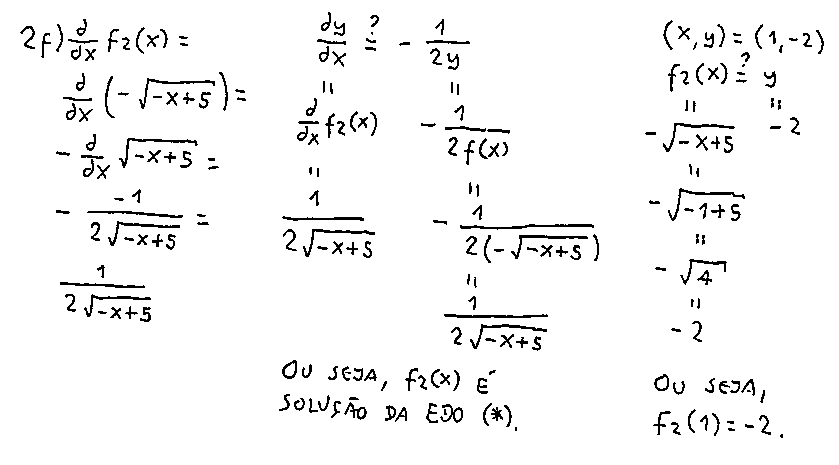
\includegraphics[height=4cm]{2020-2-C2/20210502_C2_P2_2f.pdf}
 \end{array}
$


%\printbibliography

\GenericWarning{Success:}{Success!!!}  % Used by `M-x cv'

\end{document}

%  ____  _             _         
% |  _ \(_)_   ___   _(_)_______ 
% | | | | \ \ / / | | | |_  / _ \
% | |_| | |\ V /| |_| | |/ /  __/
% |____// | \_/  \__,_|_/___\___|
%     |__/                       
%
% «djvuize»  (to ".djvuize")
% (find-LATEXgrep "grep --color -nH --null -e djvuize 2020-1*.tex")

 (eepitch-shell)
 (eepitch-kill)
 (eepitch-shell)
# (find-fline "~/2020.2-C2/")
# (find-fline "~/LATEX/2020-2-C2/")
# (find-fline "~/bin/djvuize")

cd /tmp/
for i in *.jpg; do echo f $(basename $i .jpg); done

f () { rm -fv $1.png $1.pdf; djvuize $1.pdf }
f () { rm -fv $1.png $1.pdf; djvuize WHITEBOARDOPTS="-m 1.0" $1.pdf; xpdf $1.pdf }
f () { rm -fv $1.png $1.pdf; djvuize WHITEBOARDOPTS="-m 0.5" $1.pdf; xpdf $1.pdf }
f () { rm -fv $1.png $1.pdf; djvuize WHITEBOARDOPTS="-m 0.25" $1.pdf; xpdf $1.pdf }
f () { cp -fv $1.png $1.pdf       ~/2020.2-C2/
       cp -fv        $1.pdf ~/LATEX/2020-2-C2/
       cat <<%%%
% (find-latexscan-links "C2" "$1")
%%%
}

f 20210502_C2_P2_1a
f 20210502_C2_P2_1b
f 20210502_C2_P2_1c
f 20210502_C2_P2_2a
f 20210502_C2_P2_2b
f 20210502_C2_P2_2c
f 20210502_C2_P2_2d
f 20210502_C2_P2_2e
f 20210502_C2_P2_2f



%  __  __       _        
% |  \/  | __ _| | _____ 
% | |\/| |/ _` | |/ / _ \
% | |  | | (_| |   <  __/
% |_|  |_|\__,_|_|\_\___|
%                        
% <make>

 (eepitch-shell)
 (eepitch-kill)
 (eepitch-shell)
# (find-LATEXfile "2019planar-has-1.mk")
make -f 2019.mk STEM=2020-2-C2-P2 veryclean
make -f 2019.mk STEM=2020-2-C2-P2 pdf

% Local Variables:
% coding: utf-8-unix
% ee-tla: "c2m202p2"
% End:
